% Szablony LaTeX dla przestrzeni fazowej HJSW (3D)

% Przykład 1: Pojedynczy przekrój 3D dla tau = 0.25 fm/c (dims vs pr)
\begin{figure}[htbp]
    \centering
    \begin{subfigure}[b]{0.48\textwidth}
        \centering
        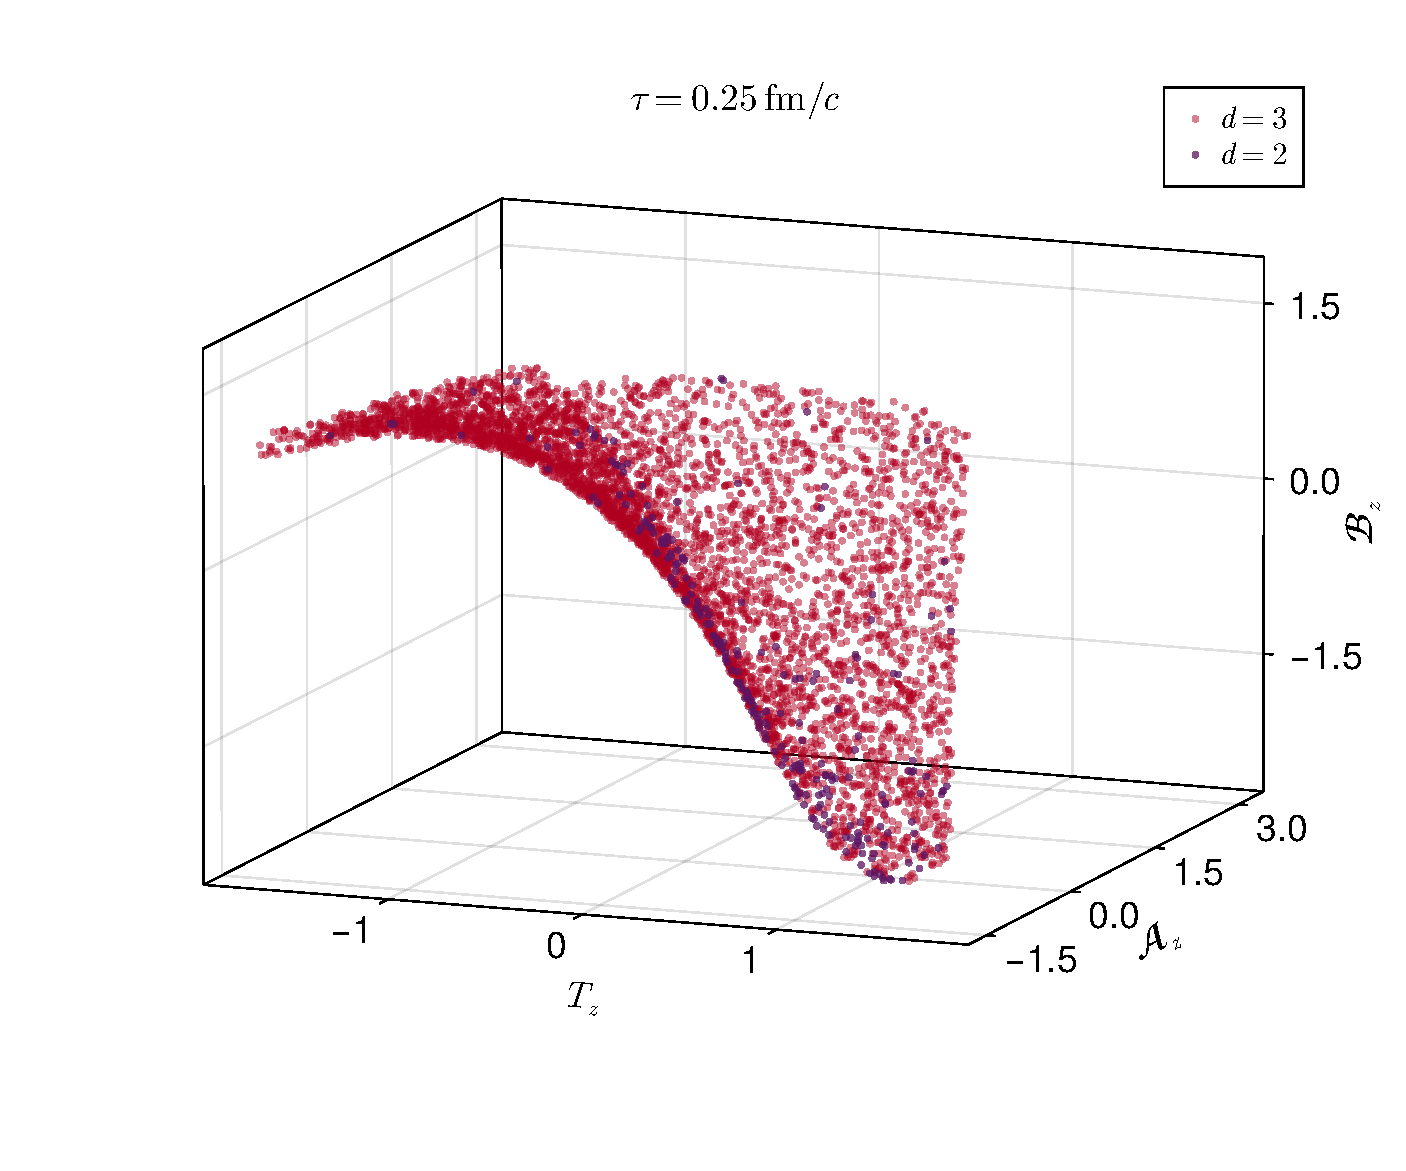
\includegraphics[width=\linewidth]{phase_space/hjsw/hjsw_zscore_slice_tau_0.25_dims.pdf}
        \caption{HJSW: \emph{dims} ($\tau = 0.25\,\mathrm{fm}/c$)}
    \end{subfigure}
    \hfill
    \begin{subfigure}[b]{0.48\textwidth}
        \centering
        \includegraphics[width=\linewidth]{phase_space/hjsw/hjsw_zscore_slice_tau_0.25_pr.pdf}
        \caption{HJSW: \emph{pr} ($\tau = 0.25\,\mathrm{fm}/c$)}
    \end{subfigure}
    \caption{Przestrzeń fazowa HJSW 3D w chwili $\tau = 0.25\,\mathrm{fm}/c$ ukazująca powstawanie 2-wymiarowej rozmaitości pośredniej.}
    \label{fig:hjsw_phase_space_tau_025}
\end{figure}

% Przykład 2: Zestawienie 3 etapów kolapsu hierarchicznego 3 -> 2 -> 1
\begin{figure}[htbp]
    \centering
    \begin{subfigure}[b]{0.32\textwidth}
        \centering
        \includegraphics[width=\linewidth]{phase_space/hjsw/hjsw_zscore_slice_tau_0.20_dims.pdf}
        \caption{$\tau = 0.20\,\mathrm{fm}/c$ ($3\mathrm{D}$)}
    \end{subfigure}
    \hfill
    \begin{subfigure}[b]{0.32\textwidth}
        \centering
        \includegraphics[width=\linewidth]{phase_space/hjsw/hjsw_zscore_slice_tau_0.35_dims.pdf}
        \caption{$\tau = 0.35\,\mathrm{fm}/c$ ($2\mathrm{D}$)}
    \end{subfigure}
    \hfill
    \begin{subfigure}[b]{0.32\textwidth}
        \centering
        \includegraphics[width=\linewidth]{phase_space/hjsw/hjsw_zscore_slice_tau_2.50_dims.pdf}
        \caption{$\tau = 2.50\,\mathrm{fm}/c$ ($1\mathrm{D}$)}
    \end{subfigure}
    \caption{Hierarchiczny kolaps przestrzeni fazowej HJSW $3\mathrm{D} \to 2\mathrm{D} \to 1\mathrm{D}$ w standaryzacji Z-Score.}
    \label{fig:hjsw_hierarchical_collapse_3slices}
\end{figure}
